\documentclass[handout]{beamer}

\usepackage[utf8]{inputenc} % Language and font encoding
\usepackage[icelandic]{babel}
\usepackage[T1]{fontenc}


\usepackage{tikz}
\usepackage[listings,theorems]{tcolorbox}
\usepackage{booktabs}
\usepackage{minted} %Minted and configuration
\usemintedstyle{default}

\renewcommand{\theFancyVerbLine}{\sffamily \arabic{FancyVerbLine}}
%%%%%%%%%%%
% More math
%%%%%%%%%%%
\newcommand{\Mod}[1]{\ \text{mod}\ #1}

%%%%%%%%%%%%%%%%%%%%%%
% Beamer configuration
%%%%%%%%%%%%%%%%%%%%%%
\setbeamertemplate{navigation symbols}{}
\usecolortheme{dove}
\setbeamercolor{frametitle}{fg=white}

\usebackgroundtemplate%
{%
\vbox to \paperheight{

\includegraphics[width=\paperwidth]{Pics/hi-slide-head-2016}

\vfill
\hspace{0.5cm}
\includegraphics[width=0.3\paperwidth]{Pics/hi-von-logo}
\vspace{0.4cm}
    }%
}

\AtBeginSection[]
{
  \begin{frame}<beamer>
    \frametitle{Yfirlit}
    \tableofcontents[currentsection]
  \end{frame}
}

\setbeamerfont{frametitle}{size=\normalsize}
\addtobeamertemplate{frametitle}{}{\vspace*{0.5cm}}

%%%%%%%%%%%%%%%%%%%%%%%%%
% tcolorbox configuration
%%%%%%%%%%%%%%%%%%%%%%%%%

% Setup from: http://tex.stackexchange.com/a/43329/21638
\tcbset{%
    noparskip,
    colback=gray!10, %background color of the box
    colframe=gray!40, %color of frame and title background
    coltext=black, %color of body text
    coltitle=black, %color of title text 
    fonttitle=\bfseries,
    alerted/.style={coltitle=red, colframe=gray!40},
    example/.style={coltitle=black, colframe=green!20, colback=green!5},
}


%%%%%%%%%%%%%%%%%%%%%%%
% Further configuration
%%%%%%%%%%%%%%%%%%%%%%%
\hypersetup{colorlinks=true,pdfauthor={Eirikur Ernir Thorsteinsson},linkcolor=blue,urlcolor=blue}
\graphicspath{{./Pics/}}

\author{Eiríkur Ernir Þorsteinsson}
\institute{Háskóli Íslands}
\date{Haust 2016}

\title{Stærðfræðimynstur í tölvunarfræði}
\subtitle{Vika 1, fyrri fyrirlestur}

\begin{document}

\begin{frame}
\titlepage
\end{frame}

\section{Um námskeiðið}

\begin{frame}{Kennari}
\begin{columns}
\column{0.5\textwidth}
\begin{itemize}
 \item Nafn: Eiríkur Ernir Þorsteinsson
 \item Aðsetur: Tæknigarði, 2. hæð, herbergi 214
 \item Tölvupóstfang: \href{mailto:eth31@hi.is}{eth31@hi.is}
 \begin{itemize}
  \item Sjá einnig: \hyperlink{frame:piazza}{Piazza}
 \end{itemize}
\end{itemize}
\column{0.5\textwidth}
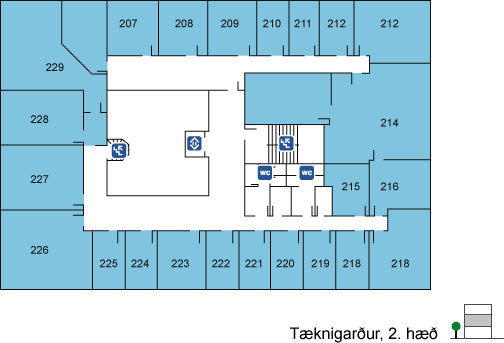
\includegraphics[width=\linewidth]{taeknigardur}
\end{columns}
\end{frame}

\begin{frame}{Tímar}
\begin{itemize}
 \item Fyrirlestrar
 \begin{itemize}
  \item Þriðjudögum klukkan 15:00 í HT-105, föstudögum klukkan 8:20 í HT-102
  \item Fyrirlestrar fara hratt yfir efni bókarinnar
 \end{itemize}
 \item Dæmatímar
 \begin{itemize}
  \item Hefjast í næstu viku
  \item Sjö hópar, miðvikudögum til föstudaga
  \begin{itemize}
   \item Einungis þarf að mæta í \emph{einn}
  \end{itemize}
  \item Hópum verður úthlutað fljótlega\textsuperscript{\textregistered}
 \end{itemize}
\end{itemize} 
\end{frame}

\begin{frame}{Námsmat}
Einkunn ákvarðast af prófseinkunn og vetrareinkunn
\begin{columns}
\column{0.5\textwidth}
\begin{itemize}
 \item Prófseinkunn skiptist í lokaprófseinkunn og miðmisserisprófseinkunn
 \item Lokaprófseinkunn er 50\% og miðmisserisprófseinkunn 20\%
 \item Undantekning: lokaprófseinkunn gildir 70\% sé hún hærri en miðmisserisprófseinkunn, sem gildir þá 0\%
\end{itemize}
\column{0.5\textwidth}
\begin{itemize}
 \item Vetrareinkunn skiptist í skilaverkefnaeinkunn og tímaverkefnaeinkunn
 \item Skilaverkefnaeinkunn gildir 20\% af heildareinkunn
 \item Tímaverkefnaeinkunn gildir 10\% af heildareinkunn
 \item Nauðsynlegt er að skila a.m.k. 6 af fyrstu 8 skilaverkefnunum!
\end{itemize}
\end{columns}
\end{frame}

\begin{frame}{Álag}
Námskeiðið er $8 ECTS$ einingar. 60 ECTS einingar eru skilgreindar sem 1500-1800 klst. af vinnu.
\[
\text{60 ECTS = 1650 klst.} \Longleftrightarrow \text{8 ECTS = 220 klst.}
\]
Misserið er 14 vikur, svo gera má ráð fyrir 15-16 klst. af vinnu í viku. Þar af eru 4 klst. í fyrirlestrum og dæmatímum.
\end{frame}

\section{Námefni og tól}

\begin{frame}{Kennslubók námskeiðsins}
\begin{columns}
\column{0.5\textwidth}
\begin{itemize}
 \item Nokkrar leiðir til að nálgast kennslubók og tilheyrandi efni
 \begin{itemize}
  \item Kaupa bók úr pappír (fæst í Bóksölu stúdenta), vefbók og æfingaaðgangur fylgir með
  \item Kaupa vefbók og æfingaaðgang á vefsíðu
  \item Kaupa æfingaaðgang eingöngu
 \end{itemize}
\end{itemize}
\column{0.5\textwidth}
\begin{center}
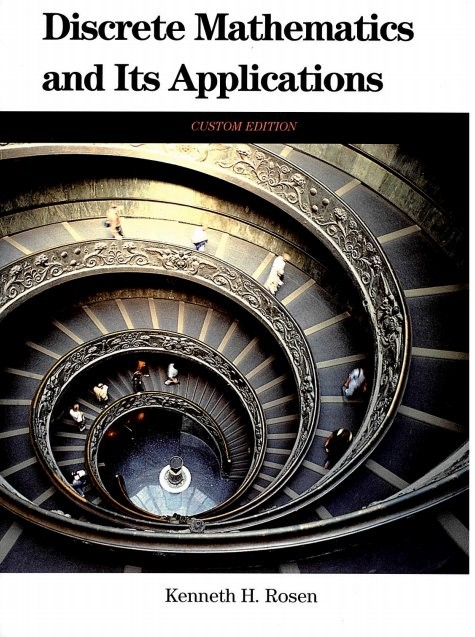
\includegraphics[width=0.7\linewidth]{Pics/rosen}
\end{center}
\end{columns}
\end{frame}

\begin{frame}{Connect}
\begin{itemize}
 \item Kennslusíða bókarinnar, \href{http://connect.mheducation.com/class/tol104g16}{McGraw-Hill Connect} verður notuð í dæmatímum og fyrirlestrum
 \begin{itemize}
  \item Inniheldur æfingaverkefni
  \item Athugið að kaupa þarf aðgang!
 \end{itemize}
\end{itemize}
\end{frame}

\begin{frame}{Gradescope}
\begin{itemize}
 \item Verkefnaskil fara fram í vefkerfinu \href{https://gradescope.com/}{Gradescope}
 \item Aðgangskóði er \textbf{926WD9}
 \item Kerfið tekur við \texttt{.pdf} skrám
 \item Fyrstu skilin verða í næstu viku
\end{itemize}
\end{frame}

\begin{frame}{Fyrirspurnir og umræður}
\label{frame:piazza}
\begin{itemize}
 \item Spjallkerfið \href{https://piazza.com/hi.is/fall2016/tol104g}{Piazza} verður notað í þessu námskeiði
 \item Kerfið mun vera besta leiðin til að fá svör frá samnemendum, dæmatímakennurum og undirrituðum
 \item Setjið allar fyrirspurnir um námskeiðið þangað!
 \begin{itemize}
  \item Kemur í stað tölvupósts
 \end{itemize}
\end{itemize}
\end{frame}

\subsection{Heilræði}

\begin{frame}{Heilræði}
\pause
\begin{itemize}
 \item Takið þátt í tímum\pause
 \item Gerið dæmin \pause
 \item Nýtið aðstoð 
 \begin{itemize}
  \item Piazza!
  \item Nemendafélög og lengra komnir nemar
  \item Námsráðgjöf HÍ \pause
 \end{itemize}
 \item Sofið og slakið á
\end{itemize}
\end{frame}

\section{Yrðingar}

\begin{frame}{Yrðingar}
\begin{tcolorbox}[title=Yrðing]
Yrðing (e. \emph{proposition}) er fullyrðing sem er áreiðanlega sönn eða ósönn.
\end{tcolorbox}
\begin{columns}
\column{0.6\textwidth}
\begin{itemize}
 \item Dæmi um yrðingar:
 \begin{itemize}
  \item Við erum stödd í stofu HT-105
  \item $2 + 2 = 4$
  \item $1 + 2 = 5$
 \end{itemize}
\end{itemize}
\column{0.4\textwidth}
\begin{itemize}
 \item Ekki dæmi um yrðingar:
 \begin{itemize}
  \item Lokaðu hurðinni!
  \item Hvað er klukkan?
 \end{itemize}
\end{itemize}
\end{columns}
\end{frame}

\begin{frame}{Yrðingar}
\begin{tcolorbox}[title=Yrðing]
Yrðing (e. \emph{proposition}) er fullyrðing sem er áreiðanlega sönn eða ósönn.
\end{tcolorbox}
\begin{itemize}
 \item Ekki yrðingar (órætt)
 \begin{itemize}
  \item $x + 1 = 2$
  \item $x + y = z$
 \end{itemize} \pause
 \item Mætti breyta þessu í yrðingar?\pause
 \begin{itemize}
  \item Já, með því að gefa breytunum $x$, $y$ og $z$ gildi
 \end{itemize}
\end{itemize}
\end{frame}

\begin{frame}{Yrðingabreytur}
\begin{itemize}
 \item Hægt er að nota yrðingabreytur (e. \emph{propositional variables}) til að tákna yrðingar
 \begin{itemize}
  \item Alveg hliðstætt því að nota breytur til að geyma gildi á tölum
 \end{itemize}
 \item Oftast eru stafirnir $p, q, r$ og $s$ notaðir til að tákna yrðingabreytur
 \item Yrðinguna sem er alltaf sönn má tákna með $T$ eða 1, yrðinguna sem er alltaf ósönn má tákna með $F$ eða 0
 \item Hægt er að nota yrðingabreytur til að framkvæma yrðingareikninga (e. \emph{propositional calculus})
\end{itemize}
\end{frame}

\begin{frame}{Samsettar yrðingar}
\begin{itemize}
 \item Samsett yrðing (e. \emph{compound proposition}) er búin til með því að nota smærri yrðingar og rökvirkja (e. \emph{logic operators})
 \item Rökvirkjarnir og táknin sem notaðir eru fyrir þau:
 \begin{itemize}
  \item Neitun, $\lnot$ (e. \emph{negation})
  \item Og-un, $\land$ (e. \emph{conjunction})
  \item Eð-un, $\lor$ (e. \emph{disjunction})
  \item Afleiðing, $\to$ (e. \emph{implication})
  \item Jafngildi $\leftrightarrow$ (e. \emph{biconditional})
 \end{itemize}
\end{itemize}
\end{frame}

\subsection{Rökvirkjar}

\begin{frame}{Neitun}
Dæmi um neitun: Ef $p$ stendur fyrir ``við erum stödd í stofu HT-105'', þá stendur $\lnot p$ fyrir ``það er ekki svo að við séum stödd í stofu HT-105'' (sem umorða má í ``við erum ekki stödd í stofu HT-105'').

\vspace*{0.5cm}
Sanntafla (e. \emph{truth table}) neitunar:

\begin{center}
\begin{tabular}{ll}
\toprule
$p$&$\lnot p$\\
\midrule
0&1\\
1&0\\
\bottomrule
\end{tabular}
\end{center}
\end{frame}

\begin{frame}{Og-un}
\begin{columns}
\column{0.6\textwidth}
Samsett yrðing búin til með og-un er sönn þegar báðar yrðingarnar sem að henni koma eru sannar.

\vspace*{0.5cm}
Hvert er sanngildi samsettu yrðingarinnar ``við erum stödd í stofu HT-105 og við erum að læra Stærðfræðimynstur''? En yrðingarinnar ``við erum stödd í stofu HT-105 og við erum að læra Tölvutækni og samfélagið''?
\column{0.4\textwidth}
Sanntafla og-unar:
\begin{center}
\begin{tabular}{ccc}
\toprule
$p$&$q$&$p \land q$ \\
\midrule
1&1&1\\
1&0&0\\
0&1&0\\
0&0&0\\
\bottomrule
\end{tabular}
\end{center}
\end{columns}
\end{frame}

\begin{frame}{eð-un}
\begin{columns}
\column{0.6\textwidth}
Samsett yrðing búin til með eð-un er sönn þegar a.m.k. önnur yrðingin sem að henni kemur er sönn.

\vspace*{0.5cm}
Hvert er sanngildi samsettu yrðingarinnar ``við erum stödd í stofu HT-105 eða við erum að læra Tölvutækni og samfélagið''?
\column{0.4\textwidth}
Sanntafla eð-unar:
\begin{center}
\begin{tabular}{ccc}
\toprule
$p$&$q$&$p \lor q$ \\
\midrule
1&1&1\\
1&0&1\\
0&1&1\\
0&0&0\\
\bottomrule
\end{tabular}
\end{center}
\end{columns}
\end{frame}

\begin{frame}{Vandamál í daglegu tali}
\begin{itemize}
 \item Orðin ``og'' og ``eða'' eru tvíræð í daglegu tali
 \item Sé skrifað á matseðil ``með þessum rétti fylgja franskar eða hrísgrjón'', hvað þýðir það?\pause
 \begin{itemize}
  \item Væntanlega er átt við eitthvað á borð við ``með þessum rétti fylgja franskar eða hrísgrjón en ekki hvort tveggja''
  \item Einnig er væntanlega átt við að kúnninn skuli velja, frekar en að um sé að ræða yfirlýsingu sem hefur sanngildi \pause
 \end{itemize}
 \item Í stærðfræði/rökfræði: 
 \begin{itemize}
  \item Merking og-unar og eð-unar er skýr og samkvæmt sanntöflum
  \item Yrðing hefur sanngildi
  \item Til að tákna ``einn og aðeins einn'' af tveimur möguleikum má nota aðgreinda eðun (e. \emph{exclusive or})
 \end{itemize}
\end{itemize}
\end{frame}

\begin{frame}{Aðgreind eðun}
\begin{columns}
\column{0.6\textwidth}
Samsett yrðing búin til með aðgreindri eðun er sönn þegar ein og aðeins ein yrðinganna sem að henni koma er sönn. Aðgreind eðun er oft táknuð með \texttt{XOR} eða $\oplus$.

\vspace*{0.5cm}
Hvert er sanngildi samsettu yrðingarinnar ``við erum stödd í stofu HT-105 aðgreint-eða við erum að læra Stærðfræðimynstur''?
\column{0.4\textwidth}
Sanntafla \texttt{XOR}:
\begin{center}
\begin{tabular}{ccc}
\toprule
$p$&$q$&$p \oplus q$ \\
\midrule
1&1&0\\
1&0&1\\
0&1&1\\
0&0&0\\
\bottomrule
\end{tabular}
\end{center}
\end{columns}
\end{frame}

\begin{frame}{Afleiðing}
\begin{itemize}
 \item Hægt er að búa til samsetta yrðingu úr einni yrðingu sem leiðir til annarrar
 \item Táknað með $p \to q$
 \item Í mæltu máli má t.d. setja afleiðingu fram sem
 \begin{itemize}
  \item ef $p$, þá $q$
  \item $q$ ef $p$
  \item $q$ hvenær sem $p$
  \item nægjanlegt skilyrði fyrir $q$ er $p$
 \end{itemize}
\end{itemize}
\end{frame}

\begin{frame}{Aðgreind eðun}
\begin{columns}
\column{0.6\textwidth}
Samsetta yrðingin $p \to q$ er ósönn þegar $p$ er sönn og $q$ er ósönn, annars er hún sönn.

\vspace*{0.5cm}

Hver eru möguleg sanngildi yrðingarinnar ``ef ég er kosinn, þá mun ég lækka skatta''?

\column{0.4\textwidth}
Sanntafla afleiðingar:
\begin{center}
\begin{tabular}{ccc}
\toprule
$p$&$q$&$p \to q$ \\
\midrule
1&1&1\\
1&0&0\\
0&1&1\\
0&0&1\\
\bottomrule
\end{tabular}
\end{center}
\end{columns}
\end{frame}

\begin{frame}{Tvískilyrðing}
\begin{itemize}
 \item Hægt er að búa til samsetta yrðingu sem táknar tvískilyrðingu
 \item Táknað með $p \leftrightarrow q$
 \item Á mæltu máli má t.d. setja tvískilyrðingu fram sem
 \begin{itemize}
  \item $p$ er nauðsynlegt og nægjanlegt fyrir $q$
  \item ef $p$ þá $q$ og öfugt
  \item $p$ ef og aðeins ef $q$
  \item $p$ þá og því aðeins að $q$
 \end{itemize}
\end{itemize}
\end{frame}

\begin{frame}{Tvískilyrðing í daglegu tali}
\begin{itemize}
 \item Tvískilyrðing eru oft áskilin í daglegu tali
 \item ``Ef þú klárar aðalréttinn mátt þú fá ís'' \pause
 \item Hér er líklega átt við ``Þú mátt fá ís þá og því aðeins að þú klárir aðalréttinn''
\end{itemize}
\end{frame}

\begin{frame}{Sanntafla tvískilyrðingar}
\begin{center}
Sanntafla tvískilyrðingar
\begin{tabular}{cccccc}
\toprule
$p$&$q$&$p \to q$&$q \to p$&$p \leftrightarrow q$&$(p \to q) \land (q \to p)$\\
\midrule
1&1&1&1&1&1\\
1&0&0&1&0&0\\
0&1&1&0&0&0\\
0&0&1&1&1&1\\
\bottomrule
\end{tabular}
\end{center}
\end{frame}

\subsection{Sísönnur, mótsagnir og jafngildi}

\begin{frame}{Sísönnur og mótsagnir}
Við getum skilgreint hugtök sem tengjast samsettum yrðingum:

\begin{tcolorbox}[title=Sísanna]
Samsett yrðing sem er sönn óháð sanngildi grunnyrðinganna er kölluð sísanna (e. \emph{tautology})
\end{tcolorbox}

\begin{tcolorbox}[title=Mótsögn]
Samsett yrðing sem er \textbf{ó}sönn óháð sanngildi grunnyrðinganna er kölluð mótsögn (e. \emph{contradiction})
\end{tcolorbox}
\end{frame}

\begin{frame}{Jafngildi}
Við getum búið til skilgreiningu á því hvenær tvær yrðingar eru ``eins'':

\begin{tcolorbox}[title=Jafngildi]
Yrðingarnar $p$ og $q$ eru jafngildar (e. \emph{equivalent}) sé $p \leftrightarrow q$ sísanna.
\end{tcolorbox}

Jafngildi er oft táknað með $\equiv$.
\end{frame}


\begin{frame}{Sanntöflur og jafngildi}
Athugum hvort að $p \to q$ og $\lnot p \lor q$ séu jafngildar. Notum einn dálk fyrir hverja breytu og einn dálk fyrir hverja aðgerð. \pause
\begin{center}
\begin{tabular}{ccccc}
\toprule
$p$&$q$&$\lnot p$&$\lnot p \lor q$&$p \to q$ \\
\midrule
1&1&0&1&1\\
1&0&0&0&0\\
0&1&1&1&1\\
0&0&1&1&1\\
\bottomrule
\end{tabular}
\end{center}
Sjáum að síðustu tveir dálkarnir eru eins, svo $(p \to q) \leftrightarrow (\lnot p \lor q)$ er sísanna og þar með $p \to q \equiv \lnot p \lor q$.
\end{frame}

\begin{frame}{Forgangur rökvirkja}
Hægt er að gera forgang rökvirkja ljósan með því að nota sviga. Séu svigar ekki til staðar er forgangurinn eftirfarandi:

\begin{center}
\begin{tabular}{cc}
\toprule
Virki&Forgangur\\
\midrule
$\lnot$&1\\
$\land$&2\\
$\lor$&3\\
$\to$&4\\
$\leftrightarrow$&5\\
\bottomrule
\end{tabular}
\end{center}

Virkja ofar í töflunni skal gilda á undan þeim sem eru neðar.
\end{frame}

\begin{frame}{Næst}
Í næsta tíma verður farið yfir hagnýtingar á yrðingum (kafli 1.2), meira um jafngildi (kafli 1.3) og magnara (kafli 1.4).
\end{frame}


\end{document}
